\subsection*{Arquitetura e Protocolos 5G}
A quinta geração de comunicações móveis celulares, o 5G, representa um avanço tecnológico sem precedentes, desenhado para revolucionar não apenas o setor de telecomunicações, mas a sociedade como um todo [1].

Essa geração foi projetada com o objetivo central de entregar taxas de dados substancialmente mais rápidas, conectividade mais confiável, cobertura aprimorada e latências rigorosamente baixas em comparação com as tecnologias predecessoras [2, 3].

As especificações de desempenho técnico e as diretrizes de avaliação da nova interface de rádio foram fundamentadas pelo padrão internacional conhecido como IMT-2020, concebido e monitorado pela União Internacional de Telecomunicações (ITU) [4, 5].

Para satisfazer a gama diversificada de requisitos estipulados no IMT-2020, o 3GPP (Third Generation Partnership Project) padronizou a tecnologia em sucessivos lançamentos, denominados de "Releases", definindo toda a arquitetura física e lógica fundamental do 5G [6, 7].

O escopo operacional do 5G foi idealizado em torno de três grandes cenários de uso ou áreas de serviço, os quais são vitais para a implantação das futuras infraestruturas digitais das cidades e da indústria [8].

O primeiro desses cenários, designado como Banda Larga Móvel Aprimorada (eMBB), visa a entrega de volumes extremos de dados móveis, suportando taxas de transferência de pico teóricas que alcançam 20 Gbps no downlink e 10 Gbps no uplink [9, 10].

O segundo cenário estratégico é o de Comunicações Massivas do Tipo Máquina (mMTC), que foi minuciosamente formulado para interconectar de forma eficiente o amplo ecossistema da Internet das Coisas (IoT), suportando inúmeros dispositivos interligados que requerem extrema economia de energia e baixo custo [9, 10].

O terceiro pilar é configurado pelas Comunicações Ultra-Confiáveis e de Baixa Latência (URLLC), um arranjo vital para aplicações de controle robótico, fábricas inteligentes e processos que demandam taxas de erro na casa de $10^{-5}$ e atrasos logísticos restritos a frações de milissegundos [10, 11].

Para dar sustentação tecnológica a tamanhas exigências, a arquitetura do ecossistema 5G foi subdividida em dois grandes blocos: a Nova Rede de Acesso de Rádio (NG-RAN) e o Core de Próxima Geração (5GC) [6, 12].

\begin{figure}[ht!]
\centering
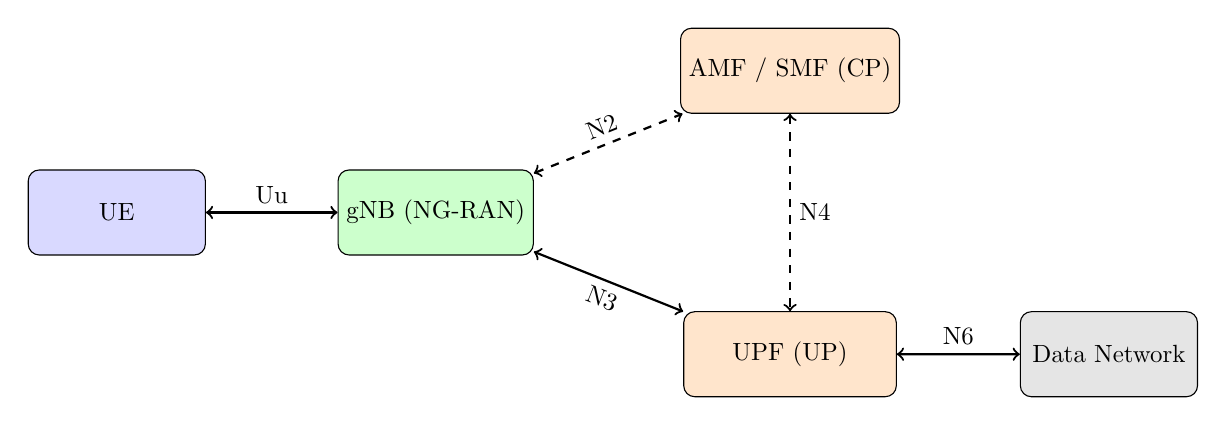
\begin{tikzpicture}[node distance=2cm, auto, scale=0.9, transform shape]
  % Nodes
  \node[draw, rectangle, rounded corners, fill=blue!15, minimum width=2.5cm, minimum height=1.2cm] (ue) {UE};
  \node[draw, rectangle, rounded corners, fill=green!20, minimum width=2.5cm, minimum height=1.2cm, right of=ue, node distance=4.5cm] (gnb) {gNB (NG-RAN)};
  \node[draw, rectangle, rounded corners, fill=orange!20, minimum width=3cm, minimum height=1.2cm, right of=gnb, node distance=5cm, yshift=2cm] (amf) {AMF / SMF (CP)};
  \node[draw, rectangle, rounded corners, fill=orange!20, minimum width=3cm, minimum height=1.2cm, right of=gnb, node distance=5cm, yshift=-2cm] (upf) {UPF (UP)};
  \node[draw, rectangle, rounded corners, fill=gray!20, minimum width=2.5cm, minimum height=1.2cm, right of=upf, node distance=4.5cm] (dn) {Data Network};

  % Edges
  \draw[<->, thick] (ue) -- node[above] {Uu} (gnb);
  \draw[<->, thick, dashed] (gnb) -- node[above, sloped] {N2} (amf);
  \draw[<->, thick] (gnb) -- node[below, sloped] {N3} (upf);
  \draw[<->, thick, dashed] (amf) -- node[right] {N4} (upf);
  \draw[<->, thick] (upf) -- node[above] {N6} (dn);
\end{tikzpicture}
\Caption{\label{fig:arquitetura_5g_short} Arquitetura Simplificada da Rede 5G (Plano de Controle e Usuário).}
\Fonte{Elaborado pelo autor.}
\end{figure}

O núcleo da rede, o 5GC, implementa o modelo de Arquitetura Baseada em Serviços (SBA), uma abordagem modernizada em que diversas funções de rede comunicam-se através de requisições de serviço em interfaces bem padronizadas [13, 14].

Esse núcleo avança significativamente em relação aos modelos prévios através da efetiva separação metodológica e estrutural do Plano de Controle e do Plano de Usuário (CUPS) [15, 16].

Impulsionado pelas capacidades do 5GC, surge o conceito inovador de Fatiamento de Rede (Network Slicing), em que a infraestrutura física de telecomunicações é dividida em incontáveis redes lógicas isoladas atuando em paralelo [17, 18].

Valendo-se do Fatiamento de Rede, cada rede virtual individual (slice) pode ser parametrizada para oferecer atributos únicos em termos de largura de banda, latência, mobilidade e segurança, enquadrando-se perfeitamente nos propósitos do cliente e na diversidade dos serviços digitais [18, 19].

\begin{figure}[ht!]
\centering
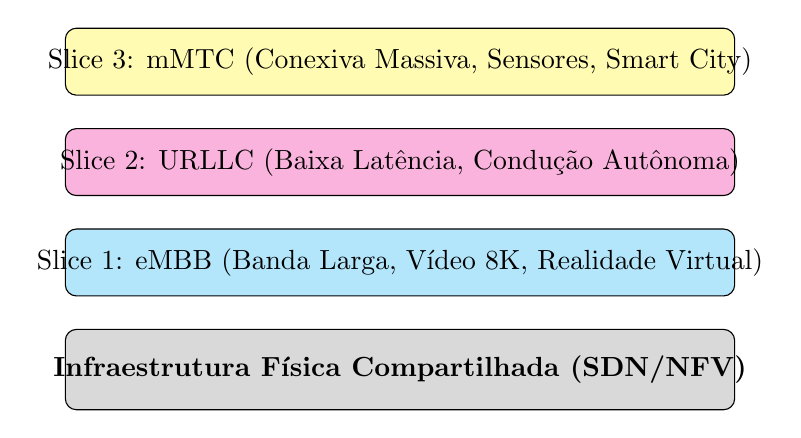
\begin{tikzpicture}[scale=0.85]
  % Infraestrutura física
  \draw[fill=gray!30, rounded corners] (0,0) rectangle (10, 1.2) node[midway, font=\bfseries] {Infraestrutura Física Compartilhada (SDN/NFV)};
  % Fatias (Slices)
  \draw[fill=cyan!30, rounded corners] (0,1.7) rectangle (10, 2.7) node[midway] {Slice 1: eMBB (Banda Larga, Vídeo 8K, Realidade Virtual)};
  \draw[fill=magenta!30, rounded corners] (0,3.2) rectangle (10, 4.2) node[midway] {Slice 2: URLLC (Baixa Latência, Condução Autônoma)};
  \draw[fill=yellow!30, rounded corners] (0,4.7) rectangle (10, 5.7) node[midway] {Slice 3: mMTC (Conexiva Massiva, Sensores, Smart City)};
\end{tikzpicture}
\Caption{\label{fig:slicing_short} Conceito de Fatiamento de Rede (Network Slicing) baseado em NFV/SDN.}
\Fonte{Elaborado pelo autor.}
\end{figure}

Essa grande flexibilidade operacional da rede e do núcleo é primariamente garantida pelas abordagens fundamentais em Redes Definidas por Software (SDN) e Virtualização de Funções de Rede (NFV) [20, 21].

A tecnologia NFV tem o papel revolucionário de abstrair as capacidades de computação e armazenamento da rede, implementando-as em software de forma ágil dentro de máquinas virtuais comerciais, dispensando a necessidade de grandes hardwares físicos proprietários [20, 22].

Em consonância, a diretriz do SDN isola a camada de dados da camada de decisões nos roteadores corporativos, consolidando de maneira eficiente as rotas a partir de um controlador unificado programável em servidor central [17, 20].

Ainda para viabilizar as baixas latências ditadas pelo URLLC, as funções e conteúdos de aplicações foram deslocados das nuvens centrais tradicionais para as extremidades locais, formando a chamada Computação de Borda de Múltiplo Acesso (MEC) [20, 23].

O emprego do MEC e a distribuição regional do elemento de núcleo UPF minimizam a dependência das onerosas ligações de longas distâncias, diminuindo o congestionamento nos datacenters centrais e melhorando a qualidade das transferências e experiências multimídia interativas [23, 24].

Quanto à infraestrutura na borda sem fio, a estação rádio base evoluiu drasticamente em relação aos antigos "eNodeB" do LTE 4G, passando a ser formalmente denominada "Next-generation Node B" ou gNodeB (gNB) [17, 25].

Esses complexos equipamentos gNBs foram desenvolvidos permitindo operações baseadas na separação rigorosa entre suas funções base: a Unidade Central (CU), responsável por processos de maior nível, e as Unidades Distribuídas (DU), localizadas mais perto da antena [26, 27].

Dada a amplitude das mudanças exigidas pela quinta geração, as operadoras elaboraram passos migratórios estratégicos, inicialmente focados na implantação baseada no modelo Não-Autônomo (NSA) [25, 28].

O modelo Não-Autônomo (NSA) ancora-se inicialmente sobre o núcleo consolidado de pacotes (EPC) do 4G, agregando portadoras e fornecendo conectividade dupla em que a torre 4G LTE atua como controladora primária enquanto a antena gNB 5G reforça vigorosamente o fluxo dos dados [25, 29].

Para finalizar a modernização, as redes se deslocam rumo ao 5G Autônomo (SA) definitivo, cenário chamado de Opção 2, em que a estação gNB se acopla livremente ao núcleo 5GC puro, concretizando funcionalidades de ponta a ponta sem qualquer arranjo residual do 4G LTE [28, 30].

Todas essas conexões via rádio com o usuário final operam utilizando uma arquitetura avançada de interface aérea global, devidamente conhecida por 5G New Radio (NR) [9, 31].

Na padronização do 5G NR, o espectro utilizável da rádio frequência sofreu uma dramática elevação das larguras de banda, dividindo as operações nos denominados Frequência Range 1 (FR1) e Frequência Range 2 (FR2) [32, 33].

O intervalo de rádio FR1 incorpora tipicamente o espectro da faixa sub-6 GHz, englobando canais em faixas que se estendem aos 7.125 GHz, o que possibilita um balanço crucial entre penetração em interiores e uma boa capacidade [34, 35].

Por outro lado, o verdadeiro salto para a massificação cibernética multicanal provém das ondas do intervalo FR2, cujas frequências, conhecidas como ondas milimétricas (mmWave), flutuam nas larguras extensas entre 24.25 GHz a 71 GHz [33, 35].

Inerente às leis físicas de transmissão nas extremas bandas milimétricas, a atenuação natural atmosférica reduz criticamente o raio geográfico alcançável das células instaladas nas torres urbanas [32, 36].

Para contornar as robustas dificuldades inerentes às altas perdas propagativas do FR2, introduziu-se obrigatoriamente a expansão dos sistemas de transmissão, implementando antenas Massivas do tipo Múltiplas Entradas e Múltiplas Saídas (Massive MIMO) [37, 38].

As estruturas compostas de Massive MIMO concentram densidades que superam dezenas de minúsculos componentes de antenas transmissoras empacotadas em um único painel [36, 39].

Valendo-se das centenas de elementos nestes painéis, a rede aplica complexos desvios de fase em tempo real para sintetizar sinais focais, num método essencial e revolucionário conceituado fisicamente como conformação de feixes ("Beamforming") [36, 40].

O Beamforming ativo dirige rigorosamente os focos das radiações milimétricas, anulando desperdícios de potência em rotas inúteis e entregando conexões muito mais eficientes ao usuário pontual e em movimento dinâmico [36, 39].

O emparelhamento do Massive MIMO permite a modulação de comunicação com múltiplos utilizadores paralelos sobre o mesmo elemento de tempo e frequência, estratégia tática estabelecida na arquitetura através do Multi-User MIMO (MU-MIMO) [37, 38].

Referente ao roteamento e espalhamento da forma de onda nos feixes, o downlink do 5G NR é fundado em bases de Multiplexação por Divisão de Frequências Ortogonais (OFDMA) para alocar os usuários nas subportadoras simultaneamente [41, 42].

Uma alteração proeminente do 5G sob a camada do OFDMA convencional é a incorporação nativa de "Numerologias", permitindo alterar geometricamente a lacuna das subportadoras em múltiplos flexíveis de 15, 30, 60 e até 120 kHz [43, 44].

Quanto maior for o espaçamento entre as referidas subportadoras do espectro OFDMA, exponencialmente mais curto o pacote ou o símbolo de duração de tempo propagado trafegará na infraestrutura aérea do ambiente radiante [45, 46].

Essa maleabilidade estrutural viabiliza os drásticos requisitos previstos pelo escopo URLLC para as aplicações sensíveis ao tempo (como na direção assistida e na telemetria rodoviária severa) que falhariam em transmissões síncronas compridas e inflexíveis [10, 45].

Em prol de garantir altíssima confiabilidade e correções de erros nessas altas taxas, o 5G NR padronizou avançados algoritmos físicos, descartando antigas formulações em favor de esquemas potentes baseados nos códigos de Paridade de Baixa Densidade, como as matrizes LDPC [47].

Combinando-se com os módulos FEC (Forward Error Correction) e LDPC, atua em paralelo o reenvio híbrido flexível de dados espaciais com confirmações automáticas HARQ (Hybrid Automatic Repeat Request) na detecção e recomposição dos sub-canais ofendidos no percurso [48].

\begin{figure}[ht!]
\centering
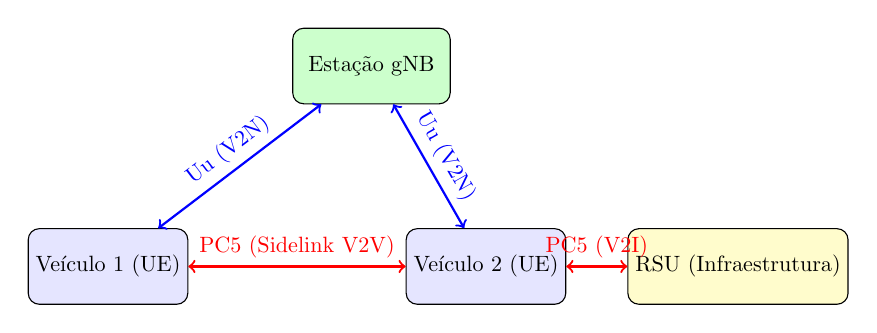
\begin{tikzpicture}[node distance=2.5cm, auto, scale=0.8, transform shape]
  % Nodes
  \node[draw, rectangle, rounded corners, fill=blue!10, minimum width=2.5cm, minimum height=1.2cm] (car1) {Veículo 1 (UE)};
  \node[draw, rectangle, rounded corners, fill=blue!10, minimum width=2.5cm, minimum height=1.2cm, right of=car1, node distance=6cm] (car2) {Veículo 2 (UE)};
  \node[draw, rectangle, rounded corners, fill=green!20, minimum width=2.5cm, minimum height=1.2cm, above right of=car1, node distance=4.5cm, xshift=1cm] (gnb) {Estação gNB};
  \node[draw, rectangle, rounded corners, fill=yellow!20, minimum width=2.5cm, minimum height=1.2cm, right of=car2, node distance=4cm] (rsu) {RSU (Infraestrutura)};

  % Edges
  \draw[<->, thick, red] (car1) -- node[above] {PC5 (Sidelink V2V)} (car2);
  \draw[<->, thick, blue] (car1) -- node[above, sloped] {Uu (V2N)} (gnb);
  \draw[<->, thick, blue] (car2) -- node[above, sloped] {Uu (V2N)} (gnb);
  \draw[<->, thick, red] (car2) -- node[above] {PC5 (V2I)} (rsu);
\end{tikzpicture}
\Caption{\label{fig:cv2x_short} Conceito 5G C-V2X abrangendo comunicações Uu (Celular) e PC5 (Sidelink direto).}
\Fonte{Elaborado pelo autor.}
\end{figure}

Desfrutando inteiramente dessa nova realidade construída com baixas latências de borda, surgem as aplicações da arquitetura C-V2X (Cellular Vehicle-to-Everything), engenhadas especificamente para orquestrar o trânsito moderno inteligente [3, 49].

As premissas baseadas em V2X no 5G impulsionam a permuta instantânea de posições geográficas entre veículos em alta velocidade, assim como entre redes veiculares cruzando sinalizações semafóricas dotadas de sensores independentes da malha civil [49, 50].

O avanço na maturação do padrão do 5G NR nas gerações pós-Release 16 impulsionou não apenas rastreamentos de frota, mas as exigentes tecnologias de "platooning" veicular avançado de automação veicular compartilhada sem intervenções do controle rodoviário humano [50, 51].

Dentro dos blocos lógicos desse segmento automotivo formidável, a pedra fundamental reside na estipulação rádio referenciada por Interface PC5, amplamente batizada na indústria pelas alcunhas de "Sidelink" [50, 52].

A capacidade "Sidelink" do 5G engendra autênticas comunicações radiais ponto a ponto orientadas de dispositivos para dispositivos (D2D) sem depender da coordenação em nuvens ou em trânsitos centrais via gNB para que os pacotes troquem de rotas cruciais [49, 50].

Ao harmonizar formidavelmente a capacidade multimegabit do feixe mmWave, o isolamento lógico das fatias NFV e as topologias diretas distribuídas em Sidelink e MEC, a quinta geração sela a base imutável para consolidar o avanço sem limites das sociedades veiculares urbanas nos anos seguintes [10, 51, 53].

Este capítulo aborda os princípios do processamento digital de sinais na interface aérea do 5G. Existem três tópicos principais. O primeiro abrange as técnicas subjacentes para transmissão e recepção que o 5G herdou dos sistemas 2G e 3G, como por exemplo, modulação, demodulação e estimativa de canal. O segundo abrange a multiplexação por divisão de frequências ortogonais (\gls{OFDMA}), uma técnica herdada do LTE através da qual a estação base pode se comunicar com diferentes dispositivos móveis simultaneamente. O terceiro abrange o gerenciamento de erros no fluxo de dados recebido por meio de correção antecipada de erro e retransmissão. Também serão discutidos uma série de problemas inerentes às elevadas frequências de rádio e que são especialmente relevantes ao 5G.

Este capítulo contém um amparo matemático maior que a maioria dos outros materiais, no entanto, foi mantido deliberadamente leve com o objetivo de tornar o estudo acessível para aqueles sem um denso embasamento em matemática avançada. A Bibliografia reúne referências chave para leitura complementar, tanto para o material explícito neste capítulo como para a matemática subjacente.

\subsection{Modulação e Demodulação}

\subsubsection{Sinal da Portadora}
Em um sistema de comunicação sem fio, a onda de rádio (vista no Capítulo 4) atua como um sinal de portadora. Matematicamente, nós podemos expressar o sinal da portadora através da seguinte função periódica: